%===================================== CHAP 3 =================================

\chapter{Related Work}
The recent advancement in virtual, augmented and mixed reality (VR/AR/MR) technologies by companies such as Oculus and Microsoft 
has contributed to the development of applications which aims to solve real world problems. The field of Computer Supported Collaborative Learning (CSCL) (see Section \ref{section:CSCL}) and Computer Supported Cooperative Work (CSCW) has according to Ens et al. over the last three decades culminated in rich theory about collaboration and how it can be more than just the sum of its parts \cite{ens2019revisiting}.

Although the use of VR/AR/MR for collaborative tasks has been studied considerably over the years, not much research has gone in the field of using VR, collaboration, design principles and tools for developing and evaluating collaborative workplace training. 

This section will review and discuss related work and then compare their respective features that are relevant for this thesis. 




\section{Collaborative VR Neurosurgical Training}
A 2007 paper by Kockro et al. describes their attempt at making a collaborative VR environment for planning and training for neurosurgery\cite{kockro2007collaborative}. This came at a time where HMDs were less accessible, so the technology is not quite the same as is used now, but still falls within the MR spectrum. This project uses an interactive console with hand- and device-tracking that allows for manipulation of 3D data. This data is then displayed with a stereoscopic projector to the rest of the team so the collaboration can take place.

Perhaps the most interesting part is that they mention they underestimated the importance of collaboration for learning, stating that "\textit{...collaboration is more important than we imagined, and that the mutual exchange of individual concepts and ideas is a real benefit...}". A previous attempt had been made without the collaborative aspect, but had not achieved the same results. This lends some credence to our initial hypothesis that the efficacy of the NAV applications could be improved were multi user functionality to be introduced. 



\section{Archaeological excavation}
In 2004 Benko et al. published a paper were they presented VITA (visual interaction tool for archaeology) an experimental collaborative mixed reality system for offsite visualisation of an archaeological dig \cite{benko2004collaborative}. The system allowed multiple archaeologists to collaborate remotely using several interaction methods including gestures to manipulate and explore a real life terrain model, see Figure \ref{fig:VITA}. The system utilised see-through HMDs (augmented reality headset) and a high resolution screen to visualise the archaeological dig sites, a fairly complex system architecture with several components. To facility collaboration between the users of the system used voice commands and hand gestures. The paper evaluated the user experience using experts in the archaeological field, stating the initial user reactions were very positive \cite{benko2004collaborative}.

However, before evaluation began participants where given an hour-long introduction and they were accompanied with an developer during the testing. This is not suitable or practical for the primary users for this thesis as the there are limitations in regards to time and other factors in regards to introduction of the application. The application should not require expert knowledge as a young job seeker or long introduction to its usage, but be intuitive and easily interpretable. Also, a critique from their system was that collaborating users should know were other users are looking.
Benko et al. explored the possibility of the VITA system to be used a learning tool and the outcome was promising as users gained deeper understanding of archaeological sites. This is very transferable to the ongoing NAV workplace projects - aiming to let young job seekers understand and be introduced different workplaces remotely.      

\begin{figure}[!h]
    \centering
    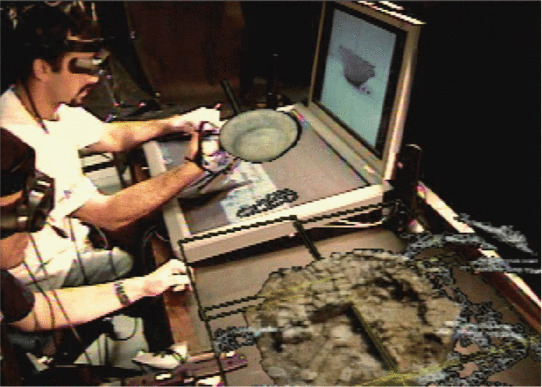
\includegraphics[width=.7\textwidth]{./fig/related_work/VITA.jpeg}
    \caption{Two users simultaneously collaborate in VITA. \cite{benko2004collaborative}}
    \label{fig:VITA}
\end{figure}


\section{Language Teaching}
The IMTEL lab has produced several master thesis in relation to VR applications. One thesis by  Morte and Skjæveland \cite{morte2019effects} is not directly relevant in regards to workplace training, but their application has features which can be beneficial for this project. The project focused on language teaching using collaborative techniques to help immigrants learn Norwegian. While their focus was on language teaching, there are still some valuable experiences to learn from, particularly when it came to the technical implementation including voice-chat and their networked multiplayer framework utilisation. Morte and Skjæveland found that distributed collaboration has potential and that the increased presence affect the motivation of the  users. Their application also included that option of having symmetric or asymmetric roles for its users, meaning one can be a student and student or student and teacher displayed as avatars in the VR environment. This can be transferred to our projects where we would have the possibility to be either a job seeker or a supervisor/mentor in the workplace training environment.     

\section{Comparison of related work}
 
Table \ref{table:comparisonRelatedWork} provides an overview the relevant features the different related work have. It is only intended to summarise the the superficial aspects of the works, and act as a guide as to where one can find information about different implementations of a feature or combination thereof, e.g. multiplayer and VR or remote workplace training.


\begin{table}[!h]
\centering
\begin{tabular}{|l|p{2cm}|p{2cm}|p{2cm}|}
\hline
                        & Neurosurgical Training    & Archaeological excavation & Language teaching \\ \hline
VR                      &                           &                           & X                 \\ \hline
Multiplayer             & /                         & /                         & X                 \\ \hline
Workplace training      &                           & X                         &                   \\ \hline
Real-world simulation   & X                         & X                         &                   \\ \hline
Voice-chat              &                           &                           & X                  \\ \hline
Co-located              & X                         & X                         & X                 \\ \hline
Remote                  &                           & X                         & X                   \\ \hline 
Symmetric role          & X                         & X                         & X                  \\ \hline 
Asymmetric role         &                           &                           & X                   \\ \hline 
\end{tabular}
\captionsetup{width=.8\linewidth}
\caption{Comparison of applications, and relevant features for each of them.
\\ ”X” = has the feature.
\\”-” = has the feature, but is limited.}
\label{table:comparisonRelatedWork}
\end{table}

\cleardoublepage